
\documentclass[a4paper,11pt]{article}

\usepackage{fontspec}
\setmainfont{Calibri}

\linespread{1}

\setlength{\oddsidemargin}{0cm}
\setlength{\evensidemargin}{0cm}
\setlength{\textheight}{23cm}
\setlength{\textwidth}{16cm}

\usepackage{amssymb,mathrsfs,algorithmic,algorithm,multirow}
\usepackage{amsmath,amsbsy,graphicx,color,url,natbib}
\usepackage{ccaption}
\setlength{\bibsep}{0.0pt}

\newcommand{\bm}{\mathbf}
\newcommand{\bs}{\boldsymbol}
\newcommand{\mt}{\mathrm}
\newcommand{\nind}{\noindent}

\usepackage{fancyhdr}
\newcommand{\tstamp}{\today}   
\lhead[\fancyplain{}{\rightmark}]       {\fancyplain{}{}}
\rhead[\fancyplain{}{\rightmark}]       {\fancyplain{}{}}
\chead[\fancyplain{}{\centermark}]       {\fancyplain{}{ENGM214 -- Process Modelling and Simulation} }
\pagestyle{fancyplain}

\usepackage{amsthm}
\theoremstyle{definition}
\newtheorem{exmp}{Example}[section]

\title{\vspace{-2cm} Lecture 3 -- Conservation principles \& constitutive relations}

\author{Tao Chen\\
{\small \emph{Department of Chemical \& Process Engineering, University of Surrey, UK}}\\
{\small (email: \texttt{t.chen@surrey.ac.uk}; \hspace{0.5cm} updated on \today )}
}
\date{}

\begin{document}
\maketitle

%\tableofcontents
\vspace{-0.5cm}

In Lecture 2, we discussed the principle of the modelling, the underlying assumptions about the system and its behaviour, 
and the systematic methodology for developing a model. In this lecture we discuss the next step, that is the development
of the describing equations. One key aspect in this process is the application of conservation principles for conserved extensive quantities. 
Another important aspect is the development of the constitutive relations which provide a set of relations which
are used to complete the model.

\section{The concept of a balance volume}

Balance volume, and in fact a lot of other concepts in process modelling, are based on \emph{thermodynamic} concepts.
The key elements of thermodynamics will be explained when needed to make this module as self-contained as possible,
but it will be very beneficial to refresh your knowledge in thermodynamics.


\subsection*{Balance volume} 

For modelling purposes, thermodynamic properties (e.g. temperature, pressure, inernal energy, and so on)
are related to a defined region of
3D space which has an associated volume $\mathcal{V}$ and surface $\mathcal{F}$. This region is usually a
volume encapsulated by a closed surface which then defines the region of interest for
the quantities of mass, energy and momentum. This is usually termed the ``balance
volume'' or ``control volume''. Associated with this volume is a volume surface, $\mathcal{F}$,
which provides a connection to the surroundings or to other defined volumes of the
process. Balance volume is also referred to as ``system'' or ``sub-system'' upon which modelling is performed.

Here we re-visit the important classification of thermodynamic properties into ``extensive'' and ``intensive'':
\begin{itemize}
	\item An \textbf{extensive} property of a system or a balance volume is a property which depends on the extent of the system.
		\begin{itemize}
			\item Examples: total mass, volume, component mass, energy or enthalpy
			\item Loosely put, extensive properties reflect the ``size'' of the system 
		\end{itemize}	
	\item An \textbf{intensive} property is one which does not depend on the extent of the system
		\begin{itemize}
			\item Examples: temperature, pressure, density, composition
			\item Loosely put, intensive properties do not reflect the ``size'' of the system			
		\end{itemize}
	\item \textbf{Conservation} (or balance) within a balance volume refers exclusively to its extensive properties
		\begin{itemize}
			\item We can talk about ``mass balance'', ``energy balance'', ``momentum balance'', ``population balance'', ...
			\item We \textbf{cannot} talk about ``temperature balance'', ``pressure balance'', ``concentration balance'', ...
		\end{itemize}	
\end{itemize}

Balance volume $\mathcal{V}$ can change in time, so can the surface $\mathcal{F}$: 
think of a rising gas bubble in a liquid being the region of interest.


\subsection*{Defining balance volume(s)}

The usual methods to help define the balance volume(s) are:
\begin{itemize}
	\item The physical equipment volumes, which define distinct regions in space which 
	contain matter or energy. For example, the volume of a reactor in the case of
	mass or in the case of energy, the walls of the vessel.
	\item The separate phases or states of aggregation in which matter is identified. This
	includes gaseous, liquid and solid states of aggregation.
\end{itemize}

Typical candidates are regions which contain only one phase and can be assumed to have a uniform flow pattern.
When alternatives exist, consider the \textbf{purpose} of modelling. For example, the required accuracy on the model output
will determine the level of detail of the model (thus e.g. whether a single balance volume with uniform temperature, 
or many small balance volumes each having different temperature). In addition, consider the required variables to be predicted
by the model -- does the chosen balance volume allow the prediction of these variables (refer to Example \ref{exmp:evap}).

\begin{exmp}[Wine fermentation]
\label{exmp:wine_ferm}
In the case of grape juice fermentation, this is normally performed in stainless steel tanks similar to those shown in Fig. \ref{fig:wine_ferm}.
Within the fermenter, we can identify three distinct phases of interest which may be
used to develop a model based on conservation of mass and energy. These phases
are vapour, juice and lees (solids).

\begin{figure} [!h]
 \begin{center}
	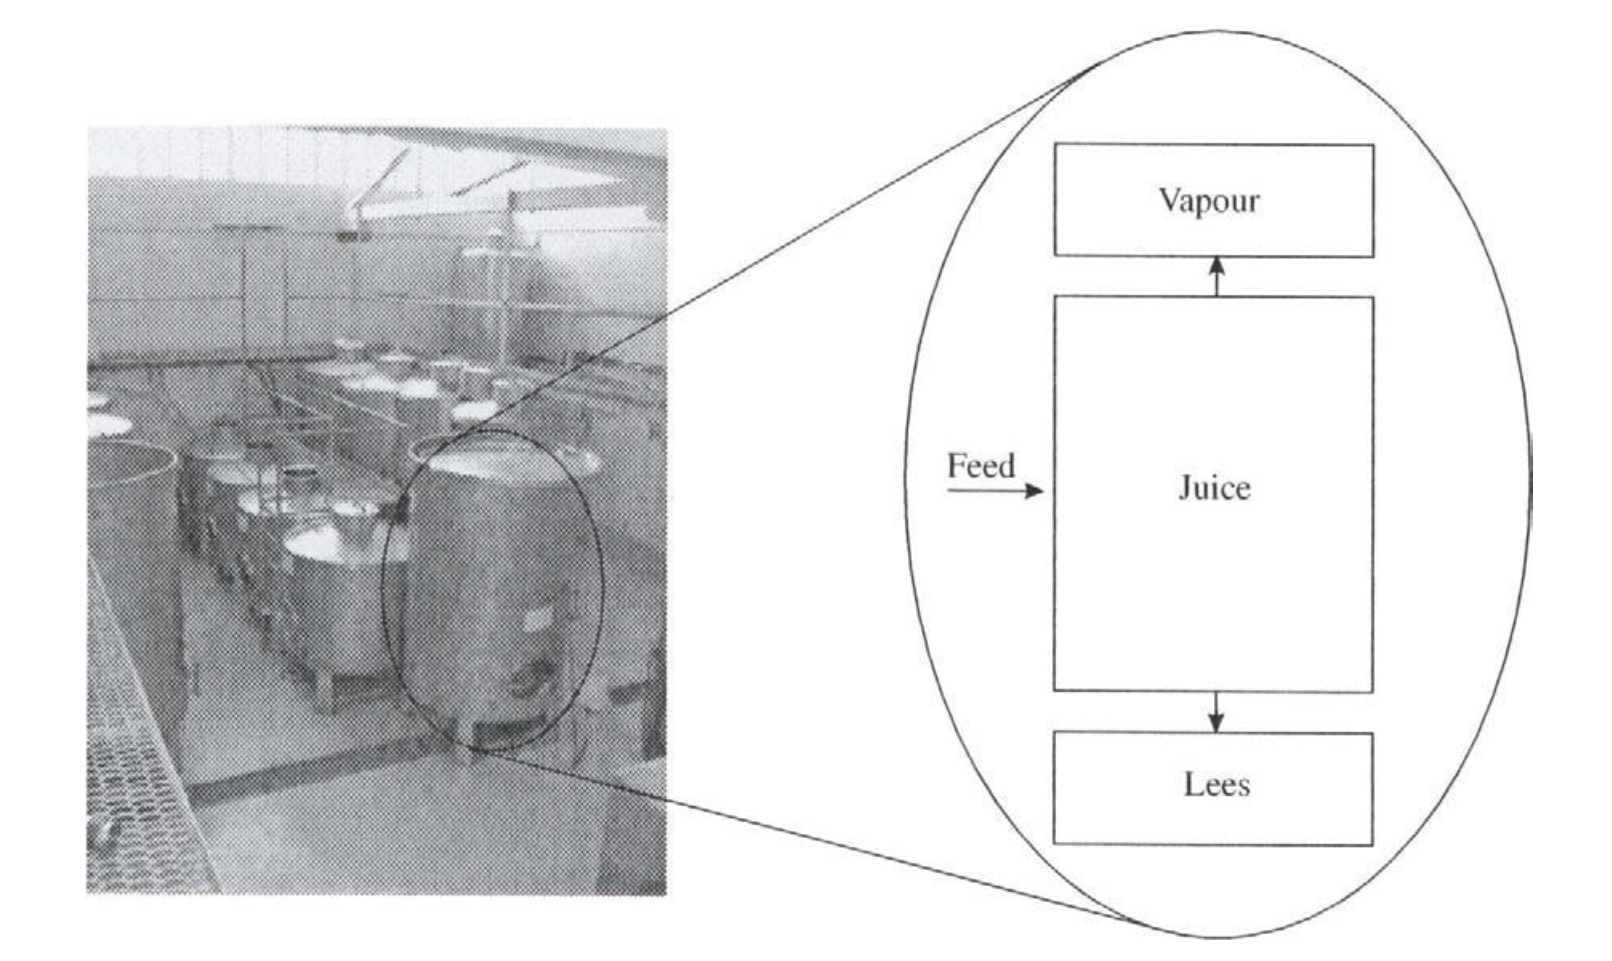
\includegraphics[width=.7\textwidth]{WineFerment}\\
 \end{center}
 \caption{Wine fermentation tank and balance volumes (also known as ``regions of interest'').} 
 \label{fig:wine_ferm}
\end{figure}

Additional information about how fermentation works can be found at this very useful link:
\url{http://encyclopedia.che.engin.umich.edu/Pages/Reactors/Bioreactors/Bioreactors.html}

\end{exmp}

\begin{exmp}[Evaporator]
\label{exmp:evap}
In a process evaporator shown in Fig. \ref{fig:evap}, we could have two choices of balance volumes.
The choice depends on the \textbf{purpose} of modelling. For example, if the model is to be used
for optimal control of the liquid level in the vessel, case (b) should be chosen.

\begin{figure} [!h]
 \begin{center}
	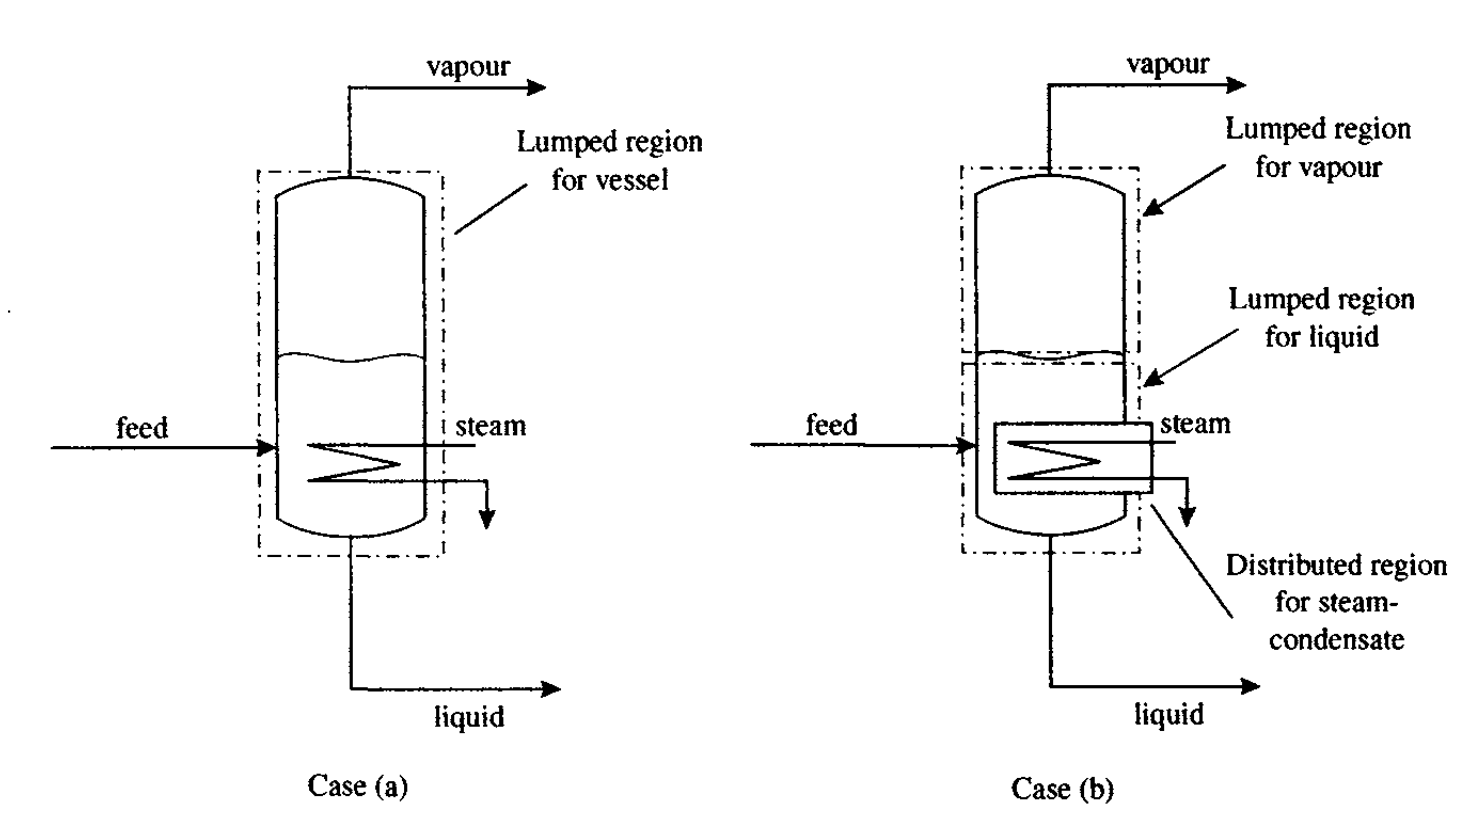
\includegraphics[width=.7\textwidth]{Evap}\\
 \end{center}
 \caption{Possible balance volumes for a process evaporator.} 
 \label{fig:evap}
\end{figure}

Information about a typical flash evaporator can be found here:
\url{https://en.wikipedia.org/wiki/Flash_evaporation}.
Note that there are many types of evaporators.

\end{exmp}


\begin{exmp}[Distillation column]
\label{exmp:dist}
A  distillation column is illustrated in Fig. \ref{fig:dist}. This is a comple system requiring multiple balance volumes.
A typical choice here is to assign one balance volume to each ``tray'' (refer to the link below for how a distillation column works),
and neighbouring balance volumes are connected by mass and/or energy flows.
The models of all balance volumes as well as the equations describing their connections together form a complete mathematic model of the entire system.

\begin{figure} [!h]
 \begin{center}
	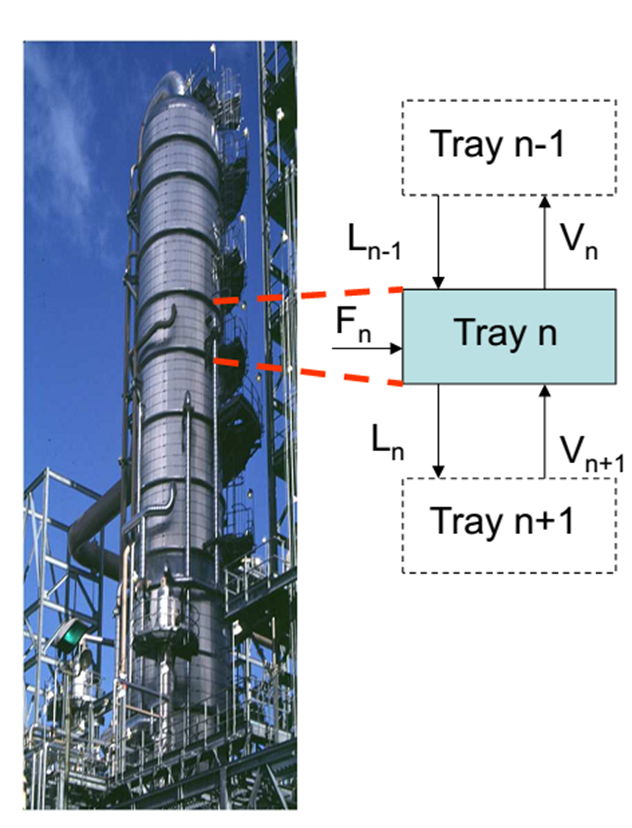
\includegraphics[width=.3\textwidth]{dist}\\
 \end{center}
 \caption{Defining balance volumes for a distillation column.} 
 \label{fig:dist}
\end{figure}

Additional information about distillation column can be found here:
\url{http://encyclopedia.che.engin.umich.edu/Pages/SeparationsChemical/DistillationColumns/DistillationColumns.html}.

\end{exmp}


\subsection*{Coordinate systems in space}

The space where a balance volume is located can be represented using 
one of the coordinate systems shown in Fig. \ref{fig:coord}, depending on the geometry of the balance volume.
The choice of coordinate system will have an impact on the modelling equations.
\begin{itemize}
	\item Cartesian or rectangular co-ordinates, where a point in space is given by the position along three co-ordinates: 
		$(x, y, z)$.
	\item Cylindrical co-ordinates, where a point is identified by a radial dimension, an angle of rotation and an axial distance: 
		$(r, \theta, z)$.
	\item Spherical co-ordinates, where the point in space is given by a radial dimension, an angle of rotation and an angle of elevation: 
		$(r, \theta, \phi)$.
\end{itemize}

\begin{figure} [!h]
 \begin{center}
	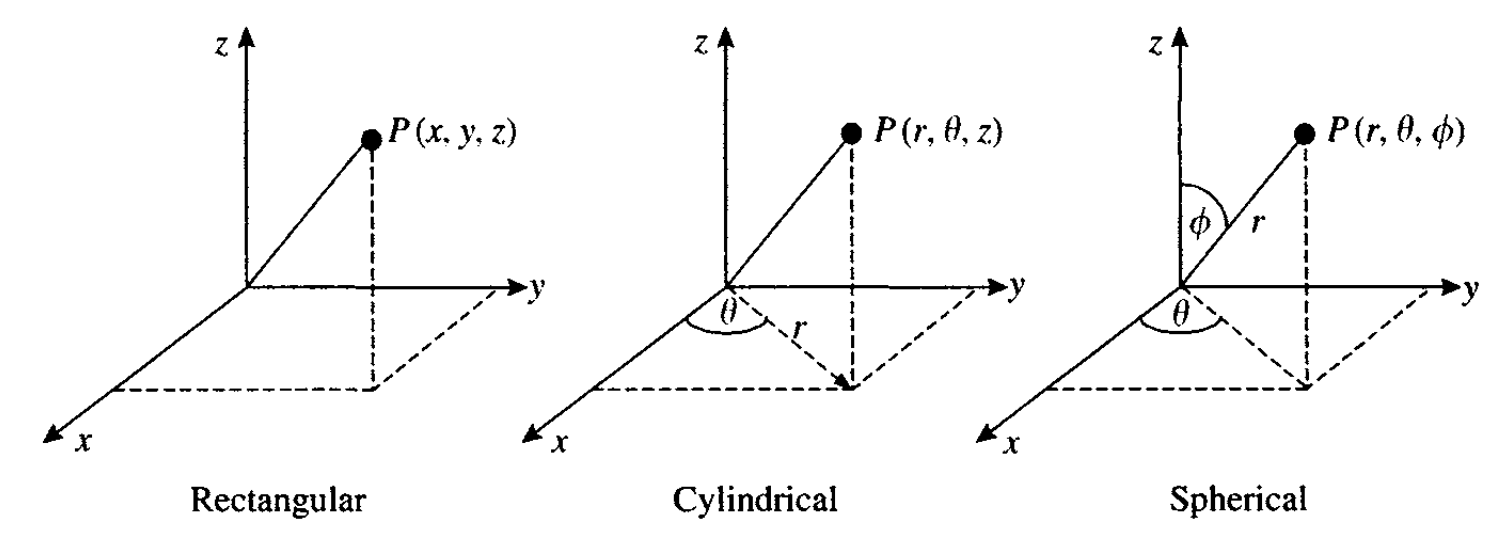
\includegraphics[width=.6\textwidth]{coord}\\
 \end{center}
 \caption{Coordinate systems.} 
 \label{fig:coord}
\end{figure}

The three coordinate systems are related. For example, one can transform the cylindrical coordinate system $(r, \theta, z)$
to the reactangular one $(x, y, z)$ by using:

\begin{equation}
	x = r \cos(\theta), \; 
	y = r \sin(\theta), \;
	z = z
\end{equation}

\noindent You should be able to derive the equations for transforming between any of the coordinate systems.

Note that we don't always need 3D modelling. In many cases, depending on the \textbf{purpose} of modelling, we can assume
that the variables of interest do not depend on a certain axis or axes, and thus the resulting model will be simplified to
2D, 1D, or even 0D (i.e. the variables do not depend on the spatial position at all, termed ``lumped parameter model'' which will be discussed later).

\begin{exmp}[Heat conduction in a column]
\label{exmp:cylin}
Suppose a mathematical model is to be developed for heat conduction, and the heat source is at the top of the column and symmetric
with respect to the axis $\theta$. Because of this symmetry, we can assume that the temperature profile
does not depend on $\theta$, but only on $r$ (the distance to the central axis) and $z$ (the vertical axis).
Therefore we can simplify the 3D cylindrical coordinate to 2D involving only $r$ and $z$.

\begin{figure} [!h]
 \begin{center}
	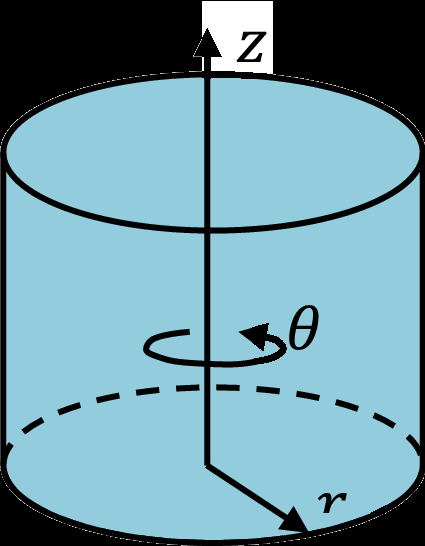
\includegraphics[width=.15\textwidth]{cylin_1} 	\hspace{1cm}
	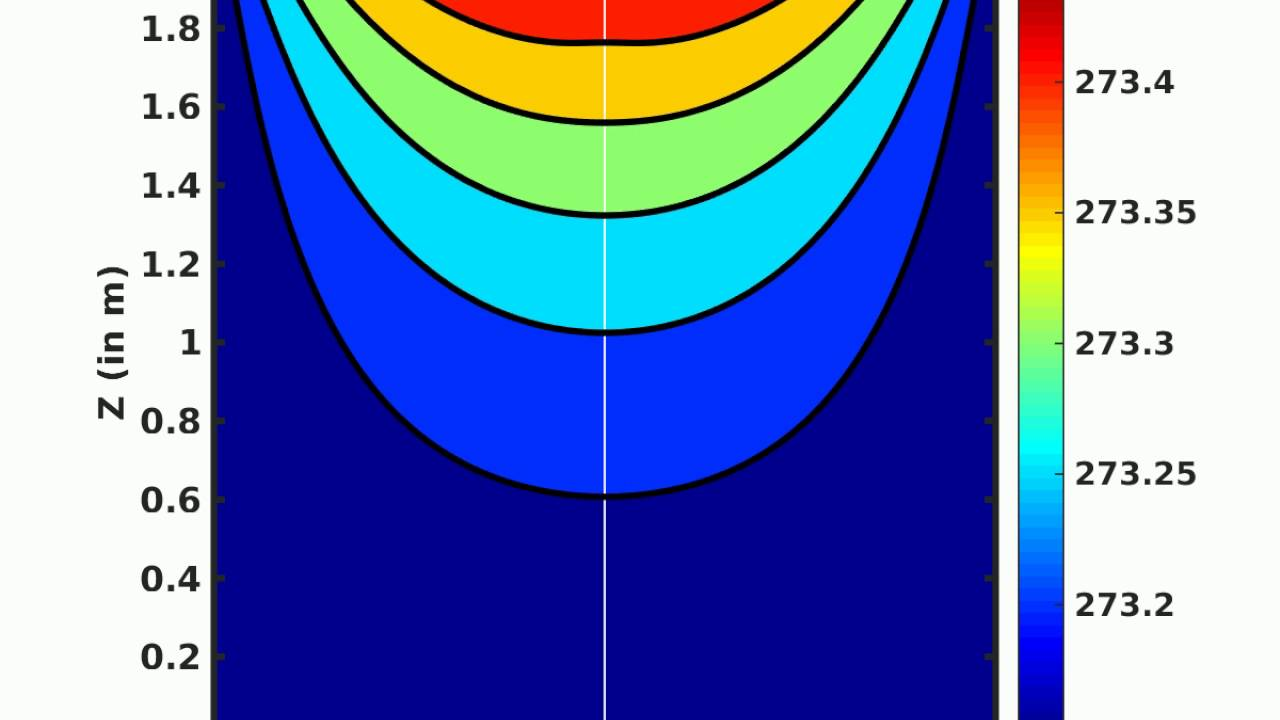
\includegraphics[width=.35\textwidth]{cylin_2}
 \end{center}
 \caption{Heat conduction in a column. Left: the 3D cylindrical coordinate; 
 	Right: model prediction of temperature profile in 2D (only dependent on $r$ and $z$.} 
 \label{fig:cylin}
\end{figure}

\end{exmp}


\begin{exmp}[Continuously stirred tank reactor (CSTR)]
\label{exmp:cstr}
In a CSTR, usually we assume that stirring is effective and thus the balance volume in the tank
is sufficiently uniform. Therefore when modelling the concentration and temperature in the tank, 
we consider the variables independent of spatial location, and thus this is a ``lumped parameter model''.

Additional information about CSTR can be found here: 
\url{http://encyclopedia.che.engin.umich.edu/Pages/Reactors/CSTR/CSTR.html}

\end{exmp}


\section{Conservation principle and equations}

As a result of the first law of thermodynamics, energy is conserved within a system,
although it may change its form. Also, both mass and momentum in the system will
be conserved quantities in any space. In general, for a given \textbf{extensive} property,
the conservation equation defined on a balance volume $\mathcal{V}$ with boundary surface $\mathcal{F}$,
shown in Fig. \ref{fig:conserv}, is

\begin{figure} [!h]
 \begin{center}
	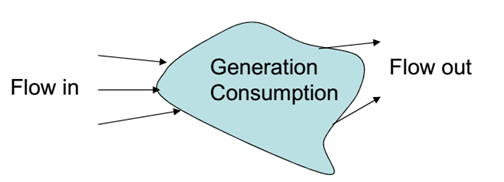
\includegraphics[width=.5\textwidth]{conserv}
 \end{center}
 \caption{Conservation of extensive properties in a balance volume.} 
 \label{fig:conserv}
\end{figure} 

\begin{align}
	\left\{ \textrm{Net change of quantity in time} \right\} &= \left\{ \textrm{Flow in through boundary} \right\} 
		- \left\{ \textrm{Flow out through boundary} \right\} \nonumber \\
		&+ \left\{ \textrm{generation} \right\}	- \left\{ \textrm{generation} \right\}	
\end{align}

The above equation can have two mathematical forms: the integral form and the derivative form. 

\subsection*{Conservation equation in integral form}

By integral form, 
we consider the total extensive quantity, $\Phi$, as the integral or sum of the volume-specific form of this property, 
$\hat{\Phi}$, 
\footnote{Loosely speaking, ``volume-specific quantity'' means to divide the total quantity by the volume. For example, if this quantity is 
mass, $m$, then the ``volume-specific mass'', $\hat{m}=m/\mathcal{V}$, will be the mass concentration in this context. Obviously
$m = \hat{m} \mathcal{V}$.
However, more rigorously speaking, this concentration may depend on the spatial location within the volume and thus the total mass
is an integration of the concentration within the volume: $m = \int_{\mathcal{V}} \hat{m} dv$.}
over the balance volume $\mathcal{V}$. Specifically consider the balance volume shown in Fig. \ref{fig:integral}, the conservation equation becomes:

\begin{figure} [!h]
 \begin{center}
	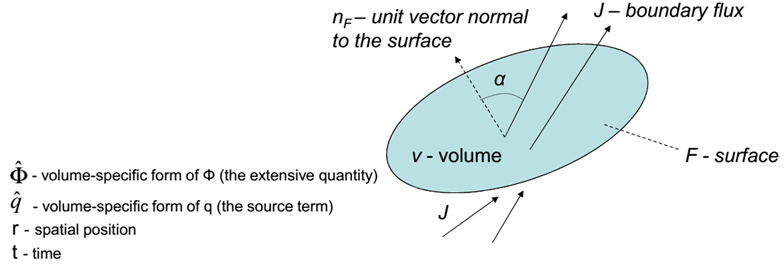
\includegraphics[width=.6\textwidth]{integral}
 \end{center}
 \caption{Illustration of the integral form of the conservation equation.} 
 \label{fig:integral}
\end{figure} 

\begin{equation} \label{eq:conserv_integral}
	\frac{d}{d t} \left\{ \int_{\mathcal{V}} \hat{\Phi} (r, t) dv \right\} = -\oint_{\mathcal{F}} J(r,t) \cdot n_{\mathcal{F}}(r) d f
		+ \int_{\mathcal{V}} \hat{q}(r, t) dv
\end{equation}

\noindent where the left-hand side represents the time variation of the extensive quantity $\Phi$ within the space $\mathcal{V}$. 
Notice that we have introduced the position vector $r$ and time $t$ to explicitly say that $\hat{\Phi} (r,t)$ is a function
of space position and time. Depending on the chosen coordinate system, $r$ can be $(x, y, z)$ (Cartesian coordinate), 
or $(r, \theta, z)$ (cylindrical coordinate), or $(r, \theta, \phi)$ (spherical coordinate).

The first term on the right-hand side accounts for the flow of $\Phi$ 
through the boundary surface $\mathcal{F}$. Here $J(r,t)$ is the flux of $\Phi$.
\footnote{For example, if $\Phi$ is mass [kg], then $J(r,t)$ is the flux of mass [kg m$^{-2}$ s$^{-1}$], where flux is defined as flow of mass per unit surface area.}
Note that the flux $J(r,t)$ is a vector with direction, e.g. the flow direction is not necessarily perpendicular to the surface, and thus we introduce
$n_{\mathcal{F}}(r)$ as the unit vector perpendicular (normal) to the surface with outward from the volume as positive direction.
Therefore, the product $J(r,t) \cdot n_{\mathcal{F}}(r)$ gives the \textbf{outward} flux of $\Phi$ perpendicular to the position $r$ on the surface
$\mathcal{F}$. Integration of this outward flux with respect to the surface gives the total flow, and since this is outward flow, a minus sign is attached.

The last term represents the net consumption or generation of the extensive quantity within the specified volume.
For simplicity consumption is treated as negative generation, thus $\hat{q}(r, t)$ represents the volume-specific \textbf{rate} of generation
of $\Phi$ within volume $\mathcal{V}$.
\footnote{For example, if $\Phi$ is mass [kg], then $q(r, t)$ is the rate of generation of mass [kg s$^{-1}$], and
$\hat{q}(r, t)$ is the rate of generation of mass per unit volume [kg m$^{-3}$ s$^{-1}$] .}
As a convention, $q(r, t)$ is also termed the ``source term'' and typically related to energy and/or chemical species generated due to reactions
and other sources.

\subsection*{Conservation equation in derivative form}

In the derivative form, the volume $\mathcal{V}$ in eq. (\ref{eq:conserv_integral}) tends to infinitely small,
resulting in\footnote{For those not familiar with vector calculus, the definition of gradient and divergence
can be found at \url{https://en.wikipedia.org/wiki/Vector_calculus_identities#Gradient}.}:

\begin{equation} \label{eq:conserv_deriv}
	\frac{\partial \hat{\Phi}}{\partial t} = - \nabla \cdot J + \hat{q}
\end{equation}

\noindent where the dependence of $J$ and $\hat{q}$ on spatial position ($r$) and time ($t$) 
is omitted to keep symbols simple. The divergence of $J$ is given by

\begin{equation} \label{eq:divg}
	\nabla \cdot J  = \textrm{div}(J) = \frac{\partial J_x}{\partial x} + \frac{\partial J_y}{\partial y} + \frac{\partial J_z}{\partial z}
\end{equation}

\noindent where $J_x$, $J_y$ and $J_z$ are three components of the flux $J$ in the direction of the coordinates $(x, y, z)$.

We will discuss the source term $q$ when we encounter specific cases. In the following, the flux term $J$, also known as ``transport term'', 
is examined in more detail.

\subsection*{Flow terms}

For process engineering application, the flux $J$ can be of two general forms:
\begin{itemize}
	\item Convective flows, $J_C$
	\item Diffusive or molecular flows, $J_D$
\end{itemize}
\noindent and they exist for mass, energy and momentum. Let's limit our discussion to the case of mass,
and we can define the two forms of flux as

\begin{align}
	J_C &= \hat{\Phi}(r, t) \; v(r, t) \label{eq:Jc} \\
	J_D &\cong -D \; \nabla \varphi(r, t) \label{eq:Jd}
\end{align}

\noindent Here the vector $v(r, t)$ refers to the convective flow into or out of the system volume $\mathcal{V}$;
it is typically the velocity componetns of the flow in the chosen coordinate system.
The diffusive flux, $J_D$, is an approximate relation involving a diffusion coefficient $D$ and the gradient of the 
potential $\varphi(r, t)$ which corresponds to the extensive property $\Phi$. For example, when considering the diffusive 
molar flow of a species we can consider the driving force or potential to be the chemical
potential of the species in the system. This is often reduced to the intensive quantity of
molar concentration of the particular species. We will illustrate these concepts through modelling examples
in a later stage.

For now, we combine eqs. (\ref{eq:conserv_deriv})(\ref{eq:Jc})(\ref{eq:Jd}) to give the general
differential form of the conservation equation:

\begin{equation} \label{eq:conserv_deriv_2}
	\frac{\partial \hat{\Phi}}{\partial t} = - \nabla \cdot \left( \hat{\Phi}(r, t) \; v(r, t) \right) 
		+ \nabla \cdot \left( D \; \nabla \varphi(r, t) \right)	 + \hat{q}
\end{equation}

\noindent If the diffusion coefficient $D$ is a constant, then above can be further simplified to
\begin{equation} \label{eq:conserv_deriv_3}
	\frac{\partial \hat{\Phi}}{\partial t} = - \nabla \cdot \left( \hat{\Phi}(r, t) \; v(r, t) \right) 
		+  D \left( \nabla^2 \varphi(r, t) \right) + \hat{q}
\end{equation}


\section{Constitutive relations}

Constitutive relations are supplementary to the conservation equations by providing models
for boundary flows and the generation and consumption phenomena, and the models of other auxiliary relations.
Mathematically, constitutive relations are represented by algebraic equations 
(as opposed to differential equations which are the common form for conservation).
Typical constitutive equations for process models can be classified as in Fig. \ref{fig:class_const}.

\begin{figure} [!h]
 \begin{center}
	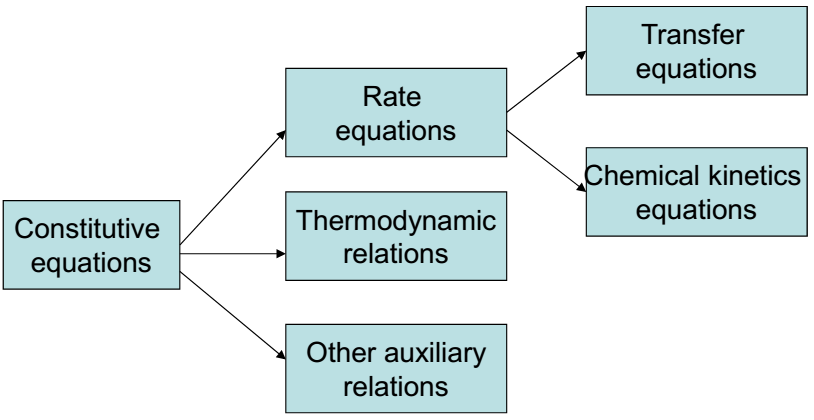
\includegraphics[width=.55\textwidth]{class_const}
 \end{center}
 \caption{Classes of constitutive equations for process models.} 
 \label{fig:class_const}
\end{figure}

\subsection{Transfer equations}

In many applications of the conservation principles for mass, energy and momentum 
there will be cases where mass, energy or momentum will be transferred into or out of
the balance volumes. This is especially the case where we deal with interacting phases
involving mass or energy. Here, there are driving forces at work which can transfer
material and energy between the phases. These driving forces are generally in terms
of the intensive properties of the system. They include concentration, temperature and
pressure differentials but can be extended to electrical potentials and other driving
forces such as chemical potential.

The generic form of the transfer equation is given by

\begin{equation} \label{eq:transfer}
	\textrm{rate}_{p \to r} = \psi ( \zeta_p - \zeta_r )
\end{equation}

\noindent where $p$ and $r$ represent two spatial positions between which the transfer occurs;
$\zeta$ is an intensive property whose gradient (difference) between $p$ and $z$ serves as the ``driving force''
for the transfer; $\psi$ is the transfer coefficient.

We now consider two cases: mass transfer and heat transfer.

\subsubsection*{Mass transfer}

Mass transfer involves a driving force in terms of chemical potential or equivalent
intensive property such as concentration or partial pressure. The fundamental concept
involves Fick's Law which describes the flux of a component ($j$) in terms of a diffusion
coefficient $D$ and a concentration gradient, $d C / d z$:

\begin{equation} \label{eq:fick}
	j = - D \frac{d C}{d z}
\end{equation}

\noindent where the typical SI units are: $j$ [kg m$^{-2}$ s$^{-1}$], $D$ [m$^2$ s$^{-1}$], $C$ [kg m$^{-3}$], $dz$ [m].

\begin{exmp}[Mass transfer between two phases]
\label{exmp:mass_transfer}
We consider mass transfer between a liquid phase and a gas phase, as ilustrated in Fig. \ref{fig:mass_transfer}.
We assume constant concentration of the species in the ``bulk'' liquid phase, $C_L$, and constant concentration in the bulk
gas phase, $C_G$. According to the two-film theory, between the two phases there exists an interface ($i$) close to which
the concentration changes linearly with spatial position; see Fig. \ref{fig:mass_transfer} 
where $d_L$ and $d_G$ are the thickness of the two films, respectively. At the interface, the concentration in the
two phases ($C_L^i$ and $C_G^i$) reaches equilibrium.

\begin{figure} [!h]
 \begin{center}
	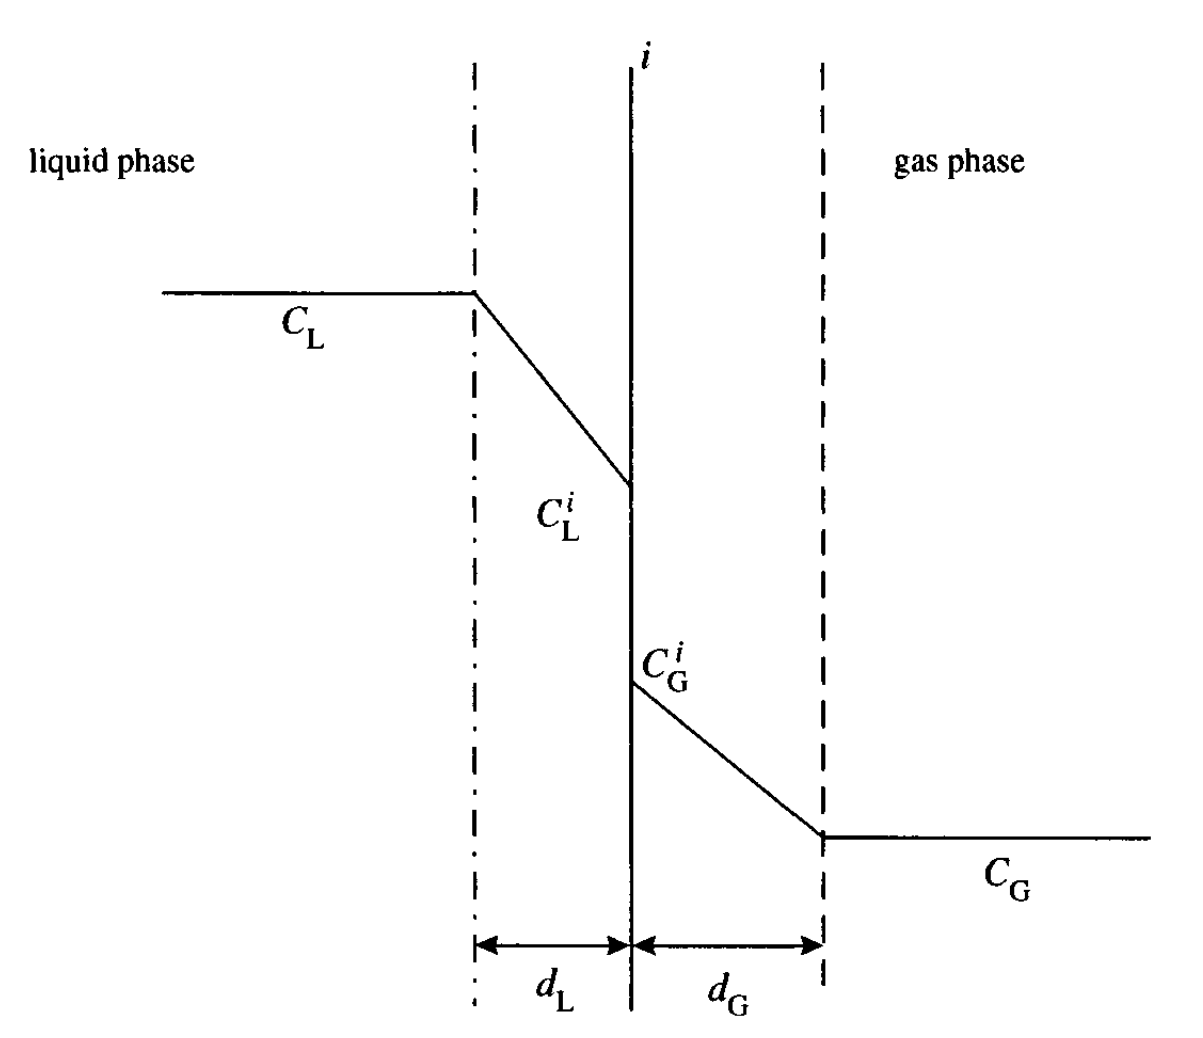
\includegraphics[width=.45\textwidth]{mass_transfer}
 \end{center}
 \caption{Two-film schematic for mass transfer between two phases.}
 \label{fig:mass_transfer}
\end{figure}

According to eq. (\ref{eq:fick}), the mass flux can be written for each side of the film and equated assuming no
accumulation at the interface to give
\begin{equation}
	j = D_L \frac{ ( C_L - C_L^i ) } { d_L } = D_G \frac{ ( C_G^i - C_G ) } { d_G}
\end{equation}

\noindent or by defining $k_L = D_L/d_L$ and $k_D = D_G/d_G$, the above can be simplified to
\begin{equation} \label{eq:diff_liq_gas}
	j = k_L ( C_L - C_L^i ) = k_G ( C_G^i - C_G )
\end{equation}

\noindent However, in the above equation the interface concentrations, $C_L^i$ and $C_G^i$, cannot be measured
and the flux should be written in terms of measurable terms. To help achieve this, we normally assume that
the species reaches equilibrium at the liquid-gas interface, i.e. $C_G^i / C_L^i = m$ where $m$ is sometimes referred to
as the species' partition coefficient between the gas and liquid phases. With this relationship and eq. (\ref{eq:diff_liq_gas}),
we can remove the interface concentrations and end up with:
\begin{equation} \label{eq:diff_liq_gas_2}
	j = K_G ( m C_L - C_G ) = K_G ( C_G^* - C_G )
\end{equation}

\noindent with
\begin{equation} 
	\frac{1}{K_G} = \frac{1}{k_G} + \frac{m}{k_L}
\end{equation}

\noindent and treating $C_G^* = m C_L$ the gas phase concentration in equilibrium with the bulk liquid phase concentration
$C_L$. Note that $C_G^*$ is generally not equl to $C_G$, and therefore $C_G^* - C_G$ is the driving force
for mass transfer betwen the liquid and gas phases. The role of $K_G$ in eq. (\ref{eq:diff_liq_gas_2}) is
of a transfer coefficient, same as $\psi$ in the generic transfer equation in eq. (\ref{eq:transfer}).

\end{exmp}

\subsubsection*{Heat transfer}

Heat transfer takes place through the three principal mechanisms: conduction, radiation and convection. 
Each mechanism can be represented by specific forms of constitutive equations. 
The following gives a brief outline of the principal heat transfer mechanisms and their mathematical representation.

\textbf{Conduction.} The rate of heat transfer by conduction is governed by the fundamental expression of
Fourier given by
\begin{equation}
	q_{CD} = -k A \frac{d T}{d x}
\end{equation}
\noindent which describes the energy transfer $q_{CD}$ [J s$^{-1}$ or W] in terms of a thermal conductivity, 
$k$ [J s$^{-1}$ m K], a heat transfer area, A [m$^2$] and a temperature gradient $dT/dx$
[K m$^{-1}$]. This general heat transfer relation can be integrated across the medium (assuming 1D between 0 and some distance $x$)
of conduction to give
\begin{equation}
	\int_0^x q_{CD} dx = -k A \int_{T_0}^{T_x} d T
\end{equation}
\noindent which results in the energy transfer between position 0 (temperature $T_0$) 
and position $x$ (temperature $T_x$):
\begin{equation}
	q_{CD} = \frac{k A}{x} (T_0 - T_x)
\end{equation}
As we can see, the heat transfer due to conduction also comforms to the general transfer equation with
temperature difference $(T_0 - T_x)$ being the driving force and a transfer coefficient.

\textbf{Radiation.} When heat is transferred from one body to another separated in space, then the key
mechanism is radiative heat transfer. This is a common mechanism in high temperature
process operations such as pyrometallurgical reactors or in steam boilers where flames
radiate energy to heat transfer surfaces. Radiation occurs from all bodies and depends
on the absolute temperature of the body and its surface properties.
For the general case of radiation between two bodies (indexed as ``1'' and ``2'') we have
\begin{equation}
	q_{R} = \sigma A_1 F_{1 \to 2} (T_1^4 - T_2^4)
\end{equation}
\noindent where $\sigma'$ is the Stefan-Boltzman constant ($5.669 \times 10^{-8} $ W m$^{-2}$ K$^{-4}$), 
$A_1$ is the surface area of body 1 [m$^2$] , and $T$ is the absolute temperature [K].
Here $F_{1 \to 2}$ is a factor to account for geometry and emissivity.
Notice that heat transfer due to radiation is due to a driving force of the difference of
temperature raised to the power of four $(T_1^4 - T_2^4)$, with a transfer coefficient.

\textbf{Convection.} Convective heat transfer occurs as a result of the transfer of energy between a moving
gas or liquid phase and a solid phase. Typical examples include the energy transfer
which occurs in process heat exchangers or in air cooled exchangers. Here, the mechanisms can be divided into natural convection and forced convection processes. In
the first case, the fluid movement is induced by density differences created by temperature gradients. In the second case, the fluid movement is a result of mechanical
motion induced by pumping action or driven by pressure differences. The rate of heat
transfer is generally expressed as
\begin{equation} \label{eq:heat}
	q_{CV} = U A \Delta T
\end{equation}
\noindent where an overall heat transfer coefficient $U$ [W m$^{-2}$ K$^{-1}$] is used together 
with a temperature driving force $\Delta T$ [K] and a heat transfer area A [m$^2$]. 

In process modelling application, we often combine conduction and convection and use the overall
heat transfer equation in eq. (\ref{eq:heat}); this implies that $U$ is calculated by considering both conduction and convection.


\subsection{Chemical kinetics}

Chemical reactions will give rise to the creation and consumption of chemical species
within the mass balance volume. Where significant heat effects accompany chemical
reaction such as the heats of reaction, these will have an impact on the related energy
balance for the balance volume.

The reaction rate is a key concept in reaction engineering. It can be defined as
the moles of species $i$ ($n_i$) generated or consumed per unit time and per unit
volume:
\begin{equation}
	r_i = \frac{1}{V} \frac{d n_i}{d t}
\end{equation}
\noindent Hence the rate at which species are generated or consumed is simply $d n_i / d t = r_i V$.

For a general reaction converting species $X$ and $Y$ into $W$ and $Z$, with the stochiometric coefficients $v_i$:
\begin{equation}
	v_x X + v_y Y \to v_w W + v_z Z,
\end{equation}
\noindent the overall reaction rate $r$ can be written in terms of the component reaction rates as
\begin{equation}
	r = \frac{1}{v_x V} \frac{d n_X}{d t} = \frac{1}{v_y V} \frac{d n_Y}{d t} 
		= - \frac{1}{v_w W} \frac{d n_V}{d t} = - \frac{1}{v_Z V} \frac{d n_Z}{d t}
\end{equation}

In general, the reaction rate for a certain species, say species $A$, will be a function of a reaction rate
constant $k_A$ and reactant species concentrations (often concentration raised to a certain power). Typical of this form would be:
\begin{equation} \label{eq:react}
	r_A = k_A \, f(C_A^m, C_B^n, \ldots)
\end{equation}
\noindent The reaction rate constant is generally temperature dependent and is written in
the form of an Arrhenius expression:
\begin{equation}
	k_A = k_0 e^{-E/(RT)}
\end{equation}
\noindent where $R$ is the universal gas constant, $E$ is the activation energy for the reaction.
Experimental data are often used to determine $k_0$ and $E$.

Finally, it's worth noting that very often, the relation between reactant concentrations and the reaction rate, i.e. eq. (\ref{eq:react}),
can be represented in the form of a power law. The order of the reaction then determines the exponent in the power law.
For example, in a reaction where species $A$ is converted:
\begin{itemize}
	\item First order reaction: $r_A = k_A C_A$
	\item Second order reaction: $r_A = k_A C_A^2$
\end{itemize}
\noindent and so on.

\subsection{Thermodynamic relations}

Thermodynamic properties are essential to process systems modelling.
In fact, they form the backbone of most successful simulations of process systems.
Nearly all process based simulation systems have extensive physical properties packages attached to them.
Typical of these are systems like ASPEN Plus. Furthermore, in stand-alone modelling and simulation applications,
we are often faced with the need to predict densities, viscosities, thermal conductivities or heat capacities for liquids, vapours and mixtures. 
In most cases, we will use simple correlations applicable to the range of validity of the model. Here we provide a selection of
thermodynamic relations that are of interest to process systems modelling. More will be discussed when encountered in specific
applications. These can be found in many classic textbooks in thermodynamics; the one in the reference list is a good option.
This link provides some useful materials for re-visiting this topic: \url{http://www.learncheme.com/screencasts/thermodynamics/textbook-SVNA-7th}.

\textbf{Single-phase relations.} These may include equations of state, such as the classic \emph{ideal gas equation} describing pressure-volume-temperature (PVT)
relations:
\begin{equation}
	P V = n R T
\end{equation}
\noindent where $P$ is system pressure [kPa], $V$ the system volume [m$^3$], $n$ is the number of moles, 
$T$ the temperature [K] and R the gas constant. More sophisticated equations are available
to handle non-ideal gases.

Another set of important relations model physical properties (e.g. density, heat capacity, enthalpy) as function of 
pressure, temperature and composition. For example the mass specific enthalpy $\hat{H}$
(enthalpy per unit mass, [J kg$^{-1}$]) can be related to temperature $T$ as follows:
\begin{equation} \label{eq:enthalpy}
	\hat{H}(T) = \hat{H}(T_R) + \int_{T_R}^T c_p(T) d T
\end{equation}
\noindent where $T_R$ is the reference temperature and $c_p$ [J kg$^{-1}$ K$^{-1}$] is the specific heat capacity. Suppose we set the reference state enthalpy
to zero ($\hat{H}(T_R)=0$ at $T_R=0$), and assume a constant $c_p$ (good approximation within a narrow temperature range) and no phase change,
the enthapy is linear in temperature: 
\begin{equation}
	\hat{H}(T) = c_p T
\end{equation}
\noindent Where the temperature change is significant, we can take this into account
through use of a temperature dependent heat capacity relationship with a polynomial:
\begin{equation}
	c_p(T) = a_0 + a_1 T + a_2 T^2 + a_3 T^3 + \cdots
\end{equation}
\noindent which can be substituted into eq. (\ref{eq:enthalpy}) for enthalpy calculation.

\textbf{Phase equilibrium equations.}
Phase equilibrium is a common assumption used in process systems modelling. In its
most fundamental form the condition relates to the \emph{equivalence} of temperature ($T$), pressure ($P$) and 
Gibbs free energy of a species $i$ ($\tilde{G}_i$) in the phases (indexed by $(1), (2), \cdots, (p)$) considered to be in equilibrium:
\begin{align}
	&T^{(1)} = T^{(2)} = \cdots = T^{(p)} \\
	&P^{(1)} = P^{(2)} = \cdots = P^{(p)} \\
	&\tilde{G}_i^{(1)} = T^{(2)} = \cdots = T^{(p)}
\end{align}
\noindent The \emph{phase equilibrium constant} has been encountered in Example \ref{exmp:mass_transfer}. Here we use
the conventional definition of this constant (also known as $K$-value) as the ratio of the mole fraction of species $i$ in the vapour
phases ($y_i$) to its mole fraction in the liquid phase ($x_i$):
\begin{equation}
	K_i = \frac{y_i}{x_i}
\end{equation}

There are many variations in calculating the $K$-value. For example, assuming ideal behaviour in both phases, the Raoult's law applies:
\begin{equation}
P = \sum_{i=1}^n x_i P_i^{\textrm{vap}}
\end{equation}
\noindent which states that the partial vapour pressure of each species of an ideal mixture of liquids, $P_j^{\textrm{vap}}$, 
is equal to the vapour pressure of the pure species multiplied by its mole fraction in the mixture. 
The vapour pressure of component $i$ can be obtained by a form of the Antoine equation:
\begin{equation}
	\ln \left( P_i^{\textrm{vap}} \right) = A_i - \frac{B_i}{T + C_i}
\end{equation}
\noindent The coefficients of the Antoine equations are listed in many standard books. 
In addition, the mole fraction of the species in the vapour phase is given by
\begin{equation}
	y_i = \frac{x_i P_i^{\textrm{vap}}}{P}
\end{equation}
\noindent. The combination of the above results in the way to calculate the $K$-value 
(essentially a partition coefficient as mentioned in Example \ref{exmp:mass_transfer}):
\begin{equation}
	K_i = \frac{y_i}{x_i} = \frac{x_i P_i^{\textrm{vap}} / P}{x_i} = \frac{P_i^{\textrm{vap}}}{P} 
\end{equation}

\subsection{Other auxiliary relations}

\textbf{Balance volume relations.} When a system being modelled involves multiple balance volumes, certain constraints may apply.
For example, in the case of the two-volume option for modelling the evaporator (Example \ref{exmp:evap}),
the volume of the reactor vessel is the sum of the volume of the liquid and vapour phases.

\textbf{Relations associated with the control system.}
These are the relations which are not originated from any physiochemical phenomena in the process, 
but which are brought about by the system which controls the process.
These include the models of individual parts of the control system and particularly the control function, 
e.g. the behaviour of the PID controller.

Furthermore, definitions directly impose relations between variables, e.g. density = mass / volume.



\begin{thebibliography}{2}
\vspace{-0.4cm}
\bibitem[{Hangos(2001)}]{Hangos2001}
	Hangos KM, Cameron IT, 2001. Process Modelling and Model Analysis, Academic Press: London.

\bibitem[{Smith(2004)}]{Smith2004}
	Smith JM, van Ness HC, Abbott MM, 2004. Introduction to Chemical Engineering Thermodynamics, 7th edition, McGraw-Hill.
\end{thebibliography}

\end{document}


